\documentclass[runningheads]{llncs}
%
\usepackage{graphicx}
\usepackage{amsmath}
\usepackage{amssymb}
\usepackage{booktabs}
\usepackage{hyperref}
\usepackage{xcolor}
\usepackage{tikz}
\usetikzlibrary{arrows.meta,positioning,fit,backgrounds,calc,shapes.geometric}
%
\begin{document}
%
\title{Defense-in-Depth for LLM Agents over Enterprise Project Databases: A Separation-of-Duties Multi-Agent Architecture for Safe Natural-Language Querying and Mutation}
%
\titlerunning{Defense-in-Depth for LLM Agents over Project Databases}
%
\author{Nguyen Trinh Quy\inst{1}\orcidID{0009-0004-8203-0736}\thanks{Corresponding author: nguyentrinhquy1411@gmail.com} \and
Tran Thanh Vu\inst{1}\orcidID{0009-0009-2165-2861} \and
Pham Nguyen Khanh Nguyen\inst{1}\orcidID{0009-0009-7619-4546} \and
Thu Le\inst{1}\orcidID{0009-0008-3480-8311}}
%
\authorrunning{N. T. Quy et al.}
%
\institute{FPT University HCM, Ho Chi Minh City, Vietnam\\
\email{\{nguyentrinhquy1411, tranthanhvu342006, nguyentvvn12\}@gmail.com}, \email{thulvm@fpt.edu.vn}}
%
\maketitle
%
\begin{abstract}
Large language model (LLM) agents that translate natural language into database queries are increasingly deployed over enterprise project-management systems such as Jira and ClickUp. The dominant ``schema-in-prompt, SQL-out'' pattern, however, fails in production along three axes: unsafe statement execution, role-based access-control (RBAC) violations that leak personally identifiable information (PII), and context/cost blow-up on large schemas. We argue that safety must be enforced by dedicated agents \emph{outside} the LLM's generation path, not by prompt instructions the model is free to ignore under adversarial input. We present \textbf{FluxBoard}, a working multi-agent system that realises this principle through a \emph{separation of duties}: a security-veto agent prunes the schema by role \emph{before} the model sees it and holds an absolute veto over the compiled query, schema pruning bounds token cost, and all data mutations are expressed as typed structured intent routed through an audited object-relational mapping (ORM) layer so the LLM never emits a mutating statement. We evaluate the architecture with a reproducible offline harness on the system's own schema, and prove a soundness property for the RBAC pre-filter: a column absent from a role's visible schema cannot be returned to that role. Against a 24-case adversarial suite spanning destructive, injection, and PII-exfiltration attacks, the defended pipeline blocks every attack within the stated threat model, where an unguarded baseline blocks none. In a model-in-the-loop study with a local LLM, an unguarded agent emits unsafe SQL for 83\% of attack prompts, and a \texttt{SELECT}-only instruction alone still leaks PII at 83\% because the forbidden column remains visible in the prompt; the full architecture reduces this to an effective data-leak rate of zero. RBAC redaction attains perfect precision and recall on the evaluated policy with no over-redaction; lexical schema pruning removes a mean 67.2\% of schema tokens on the 10-table schema, rising to 99.6\% at 300 tables, while retaining all required tables on 90\% of queries; and the safety layer adds sub-millisecond overhead, small relative to LLM inference. We are explicit about scope---results certify \emph{coverage} of the targeted threat classes rather than resistance to adaptive evasion, and lexical pruning misses joins implied by status-value semantics---and outline a model-in-the-loop adversarial study and a semantic-grounding extension as the next steps.

\keywords{LLM agents \and Text-to-SQL \and Multi-agent systems \and Access control \and Prompt injection \and Database security \and Project management}
\end{abstract}
%
\section{Introduction}
The proliferation of large language models (LLMs)~\cite{vaswani2017attention,brown2020gpt3} has reframed how non-technical staff query structured data. In modern enterprises, operational information no longer lives only in static relational warehouses; it is dispersed across dynamic project-management platforms such as Jira, ClickUp, and TaskFord, where users continuously reshape the schema through custom fields, workflow states, and real-time project partitions~\cite{jackal}. Extracting information from these systems demands fluency in specialised query languages such as the Jira Query Language (JQL), which raises a substantial barrier for non-technical users.

The natural response is an LLM agent that compiles natural-language questions into queries. The dominant implementation is deceptively simple: serialise the database schema into the prompt and ask the model to emit SQL or a domain-specific query. This ``schema-in-prompt, SQL-out'' pattern works in demonstrations but collapses in production along three axes. First, \textbf{unsafe execution}: a model that emits free-form SQL can be steered---directly or through indirect prompt injection~\cite{greshake2023injection}---into destructive \texttt{DELETE}, \texttt{DROP}, or \texttt{UPDATE} statements, or into injection through unparameterised literals~\cite{rietta}. Second, \textbf{access-control violations}: absent an enforcement boundary, the agent reads every table as though it were a system administrator, leaking PII such as member emails, audit trails, and invite secrets. Third, \textbf{context and cost blow-up}: dumping the data-definition language (DDL) of hundreds of tables into the prompt exhausts the context window and degrades reasoning, while wasting input tokens at ratios reported in the hundreds-to-one~\cite{puppygraph}.

We contend that these are not prompt-engineering problems but \emph{architectural} ones. Instructing a model to ``only generate \texttt{SELECT} statements'' is a request, not a guarantee; under adversarial input the request is precisely what fails. Safety must therefore be enforced by components that sit outside the model's generative control and cannot be talked out of their policy.

This paper presents \textbf{FluxBoard}, a working multi-agent system built on this principle of \emph{separation of duties}. Security is realised by a dedicated agent that (i) prunes the schema by the requesting user's role \emph{before} any of it reaches the model, and (ii) holds an absolute veto over the compiled query, admitting only read-only, parameterised statements. Schema pruning bounds token cost by selecting only the tables relevant to a question. Crucially, data \emph{mutations} are handled on a separate path: the LLM emits typed structured intent (e.g.\ \texttt{create\_task}), never SQL, and the intent is executed by a pre-audited ORM repository that enforces project isolation and writes an audit event for every change.

Our contributions are:
\begin{enumerate}
\item A \textbf{separation-of-duties agent architecture} in which the security boundary is a pre- and post-filter around the LLM rather than an instruction inside it (Sect.~\ref{sec:arch}).
\item \textbf{RBAC-as-schema-pruning with a soundness guarantee}: removing tables and columns by role before query compilation, so sensitive fields cannot be returned to that role even under successful prompt injection. We state and prove this as a redaction-soundness property rather than asserting it (Sect.~\ref{sec:threat}).
\item A \textbf{read-only execution veto} that enforces \texttt{SELECT}-only, blocks mutating keywords, and requires parameterised queries, neutralising injection (Sect.~\ref{sec:threat}).
\item An \textbf{ORM-only mutation path} where the model emits typed intent rather than SQL, preserving project isolation and audit logging (Sect.~\ref{sec:threat}).
\item A \textbf{reproducible evaluation} on the system's own schema quantifying attack coverage, redaction correctness, token reduction (and its growth with schema size, to 99.6\% at 300 tables), latency overhead, and mutation safety, plus a \textbf{model-in-the-loop study} on a live local LLM showing that an unguarded agent is unsafe on 83\% of attack prompts and a \texttt{SELECT}-only instruction still leaks PII at 83\%, whereas the architecture admits no data-leaking query (Sects.~\ref{sec:setup}--\ref{sec:results}), together with an honest account of where the design is conservative.
\end{enumerate}

\section{Related Work}
\textbf{Text-to-SQL and text-to-JQL.} Translating natural language to executable queries is a long-studied problem~\cite{textsql-survey,katsogiannis2023survey}, progressing from early sequence-to-sequence parsers~\cite{zhong2017seq2sql} and the cross-domain Spider benchmark~\cite{yu2018spider} to LLM prompting~\cite{rajkumar2022evaluating}, decomposed in-context pipelines~\cite{pourreza2023dinsql,gao2024dailsql}, and harder, realistic benchmarks such as BIRD~\cite{li2023bird}. Recent execution-based benchmarks expose how brittle single-shot translation remains at enterprise scale. The Jackal benchmark evaluates LLMs on text-to-JQL against a live Jira instance and shows that even frontier models, while near-perfect on verbose questions closely mirroring JQL syntax, collapse below 35\% accuracy on short or synonym-laden phrasings~\cite{jackal}. Spider~2.0 reports that a single-step GPT-4o baseline solves only $\sim$10\% of complex warehouse queries, whereas agentic systems with execution feedback exceed 70--84\%~\cite{spider2}. These results motivate decomposition and execution-grounded correction, but they target \emph{accuracy}, not the \emph{safety} of the resulting queries.

\textbf{Schema linking and pruning.} Reducing the schema presented to the model---schema linking---is known to improve both accuracy and cost on large databases~\cite{wang2020ratsql,lei2020schemalinking}, and retrieval-augmented prompting more generally conditions generation on a selected context subset~\cite{lewis2020rag}. We contribute a concrete lexical pruner (three-layer entity resolution over a foreign-key graph) and, departing from prior work that reports only accuracy, we measure its true token reduction with a standard sub-word tokenizer alongside its table-level recall, surfacing the failure modes a purely lexical approach incurs.

\textbf{LLM agents and tool use.} Tool-using agents that interleave reasoning and acting~\cite{yao2023react}, learn to invoke external tools~\cite{schick2023toolformer}, and self-correct from execution feedback~\cite{shinn2023reflexion} now underpin many data systems; recent surveys catalogue this landscape~\cite{wang2024agentsurvey}. In the database setting, decomposed architectures---planning, execution, and synthesis agents with execution-driven feedback---improve robustness on large schemas~\cite{spider2,puppygraph}, and self-correcting text-to-SQL loops re-issue failed queries using compiler feedback~\cite{ghosh}. Our work is complementary: we adopt decomposition but make the \emph{security} agent a first-class member of the pipeline with veto authority, rather than treating safety as a downstream concern.

\textbf{Prompt injection and agent security.} The risks of tool-using LLM agents---indirect prompt injection~\cite{greshake2023injection,perez2022ignore}, confused-deputy escalation, and unsafe execution---are increasingly documented, including for protocols such as the Model Context Protocol~\cite{mcp-security} and in community risk catalogues~\cite{owasp2025llm}. Mitigations in the database setting include read-only replicas and parameterised execution~\cite{rietta}. We integrate these as enforced invariants and additionally treat RBAC as a schema-level transformation applied before generation.

\textbf{Access control and injection defense.} Role-based access control is a mature model for restricting data access by user role~\cite{sandhu1996rbac,ferraiolo2001rbac}, and SQL injection has a long line of classification and countermeasure work~\cite{halfond2006sqli}. Our contribution is to fold both directly into the agent pipeline: RBAC is enforced as schema redaction \emph{before} generation, so restricted entities never enter the prompt, and injection is foreclosed by mandatory query parameterisation at the veto stage rather than by post-hoc sanitisation.

\section{System Architecture}
\label{sec:arch}
FluxBoard is a monorepo comprising a FastAPI/Python backend over a TiDB (MySQL-compatible) database accessed through SQLAlchemy, and a React frontend. The read path is coordinated by a \texttt{MasterOrchestrator} that composes four specialised agents; the mutation path is deliberately separate. Figure~\ref{fig:arch} summarises both.

\begin{figure}[htbp]
\centering
\resizebox{\textwidth}{!}{%
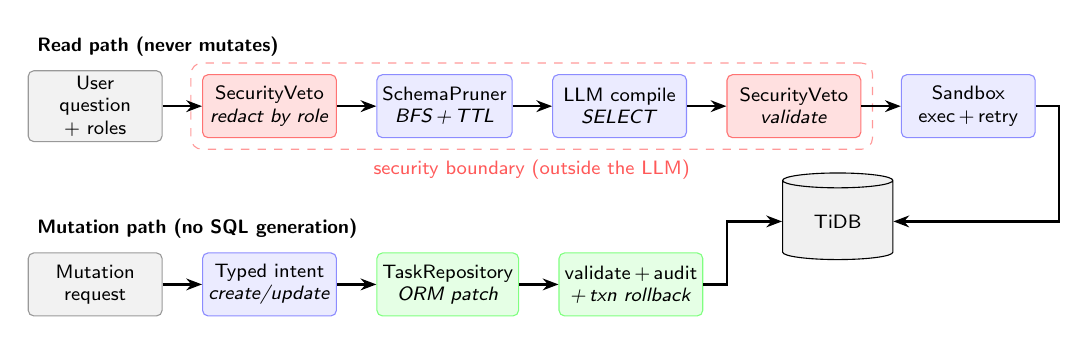
\begin{tikzpicture}[
  font=\sffamily\scriptsize,
  node distance=4mm and 5mm,
  box/.style={draw,rounded corners=2pt,minimum height=8mm,minimum width=17mm,align=center,inner sep=2pt},
  sec/.style={box,fill=red!12,draw=red!55},
  agent/.style={box,fill=blue!8,draw=blue!45},
  io/.style={box,fill=black!5,draw=black!40},
  db/.style={draw,cylinder,shape border rotate=90,aspect=0.28,fill=gray!12,minimum height=11mm,minimum width=14mm,align=center,inner sep=1pt},
  flow/.style={-{Stealth[length=2mm]},thick},
  veto/.style={-{Stealth[length=2mm]},thick,red!65},
]
% Read path (top)
\node[io] (q) {User\\question\\+ roles};
\node[sec,right=of q] (rbac) {SecurityVeto\\\textit{redact by role}};
\node[agent,right=of rbac] (prune) {SchemaPruner\\\textit{BFS\,+\,TTL}};
\node[agent,right=of prune] (llm) {LLM compile\\\textit{SELECT}};
\node[sec,right=of llm] (val) {SecurityVeto\\\textit{validate}};
\node[agent,right=of val] (exec) {Sandbox\\exec\,+\,retry};

\draw[flow] (q) -- (rbac);
\draw[flow] (rbac) -- (prune);
\draw[flow] (prune) -- (llm);
\draw[flow] (llm) -- (val);
\draw[flow] (val) -- (exec);

% Mutation path (bottom)
\node[io,below=14mm of q] (mq) {Mutation\\request};
\node[agent,right=of mq] (intent) {Typed intent\\\textit{create/update}};
\node[box,fill=green!10,draw=green!50,right=of intent] (repo) {TaskRepository\\\textit{ORM patch}};
\node[box,fill=green!10,draw=green!50,right=of repo] (guard) {validate\,+\,audit\\\textit{+\,txn rollback}};

\draw[flow] (mq) -- (intent);
\draw[flow] (intent) -- (repo);
\draw[flow] (repo) -- (guard);

% Shared DB
\node[db,right=10mm of guard,yshift=8mm] (db) {TiDB};
\draw[flow] (exec.east) -- ++(3mm,0) |- (db.east);
\draw[flow] (guard.east) -- ++(3mm,0) |- (db.west);

% labels for the two lanes
\node[anchor=west,font=\sffamily\scriptsize\bfseries] at ($(q.north west)+(0,3mm)$) {Read path (never mutates)};
\node[anchor=west,font=\sffamily\scriptsize\bfseries] at ($(mq.north west)+(0,3mm)$) {Mutation path (no SQL generation)};

% security boundary annotation
\begin{scope}[on background layer]
  \node[draw=red!40,dashed,rounded corners,fit=(rbac)(val),inner sep=4pt,label={[red!65,font=\sffamily\scriptsize]below:security boundary (outside the LLM)}] {};
\end{scope}
\end{tikzpicture}%
}
\caption{The FluxBoard architecture. Read path (top): the security-veto agent prunes the schema by role, the schema pruner selects relevant tables, the LLM compiles a parameterised \texttt{SELECT}, the veto agent validates it, and a sandboxed executor runs it with feedback-driven retry. Mutation path (bottom): the LLM emits typed structured intent routed to an audited ORM repository---never raw SQL. The security agents (red) form an enforcement boundary that sits outside the LLM's generative control.}
\label{fig:arch}
\end{figure}

\subsection{Read Path: the Orchestrator Pipeline}
For a query request carrying a question and the caller's roles, the orchestrator executes the following stages in order.

\paragraph{1. Security veto (schema redaction).} The \texttt{SecurityVetoAgent} first transforms the source schema into a \emph{role-visible} schema, dropping any table or column whose access policy excludes the caller's roles. This happens \emph{before} any schema text is constructed, so restricted entities never enter the prompt.

\paragraph{2. Schema pruning.} The \texttt{SchemaPruner} reduces the visible schema to the tables relevant to the question via three-layer entity resolution: (L1) physical table-name matching over singular/plural surface forms; (L2) a curated business-entity map (e.g.\ ``completed tasks'' $\rightarrow$ \texttt{tasks}); and (L3) column-token matching that ignores generic columns shorter than six characters to suppress noise. The resulting seed tables are expanded along foreign keys using breadth-first search (BFS) over a bidirectional key graph to recover the intermediate tables needed for joins. A time-to-live (TTL) cache memoises pruning results keyed on the question and schema fingerprint.

\paragraph{3. SQL compilation.} A compact DDL of only the selected tables, with foreign-key hints, is sent to the LLM (Groq Llama-3.3-70B) constrained to a typed \texttt{SQLOutput} structure (query, bound parameters, referenced tables, confidence, rationale). The system prompt enforces MySQL/TiDB dialect, \texttt{SELECT}-only output, and \texttt{:param} placeholders for all user values. A deterministic compiler provides a fallback when the model is unavailable or disabled.

\paragraph{4. Execution veto.} The compiled query is re-checked by the \texttt{SecurityVetoAgent} (Sect.~\ref{sec:threat}) before it can run. This is the post-filter half of the security boundary.

\paragraph{5. Sandboxed execution with feedback.} A \texttt{SpeculativeBranchAgent} executes the validated query against an isolated, read-only session identified by a three-part pointer (git commit hash, branch id, virtual environment id) and retries up to a bounded number of times on execution errors, tearing the session down afterwards.

\paragraph{6. Semantic grounding (optional).} A \texttt{JiraAnchor} component maps fuzzy entity mentions (component names, labels) to existing categorical values by cosine similarity over embeddings. In the present system the embedding provider is a deterministic, hash-based stand-in used for reproducibility; we therefore treat grounding as a described component and defer its empirical evaluation to future work (Sect.~\ref{sec:conclusion}).

\subsection{Mutation Path: Structured Intent over an ORM}
Write operations never traverse the SQL-compilation path. A natural-language mutation request is first routed---by lexical intent detection and, on miss, by an LLM constrained to a closed set of typed actions (\texttt{create\_task}, \texttt{update\_priority}, \texttt{update\_status}, \texttt{archive}, \texttt{restore})---to the corresponding method of a typed \texttt{TaskRepository}. The repository validates that any referenced status belongs to the active project, applies only the explicitly provided fields as a patch, writes an audit event, and commits within a transaction that rolls back atomically on any validation failure. Because the model emits \emph{intent} rather than SQL, the entire class of mutation-via-injection attacks is structurally absent from this path.

\section{Threat Model and Safety Mechanisms}
\label{sec:threat}
We consider an adversary who controls the natural-language input (and, by extension, any content the agent ingests that could carry indirect prompt injection) and whose goal is to (T1) execute destructive or schema-altering statements, (T2) inject SQL through unparameterised literals, or (T3) exfiltrate data the caller's role forbids. The adversary cannot modify the deployed code or bypass the API. We do \emph{not} claim to prevent the model from \emph{attempting} unsafe output; we claim that such output cannot \emph{reach} the database.

\paragraph{Read-only execution veto (T1, T2).} The post-filter validates every compiled query with three invariants: the statement must begin with \texttt{SELECT}; it must not match a mutating-keyword pattern (\texttt{DELETE}, \texttt{UPDATE}, \texttt{DROP}, \texttt{ALTER}, \texttt{INSERT}, \texttt{TRUNCATE}, \texttt{MERGE}, \texttt{CREATE}); and any user-supplied literal must be bound as a parameter rather than inlined. Violation raises a security exception and the query is never executed.

\paragraph{RBAC-as-schema-pruning (T3).} Rather than filtering results after the fact, the pre-filter removes restricted tables and columns from the schema the model is shown. A field the model never sees is a field it cannot reference; redaction is thus enforced at the schema layer and is robust to prompt injection that tries to coax the model into selecting sensitive columns. We make this precise.

\smallskip\noindent\textbf{Proposition 1 (Redaction soundness).} \emph{Let $V(r)$ be the role-visible schema derived for role $r$, and let the SQL compiler receive only the DDL of $V(r)$ as schema context. If a column $c \notin V(r)$, then any query the compiler emits for a request with role $r$ that successfully executes returns no values from $c$.}

\smallskip\noindent\emph{Proof sketch.} The compiler's sole schema context is the DDL of $V(r)$, which omits $c$. A query that reads $c$ must reference the identifier $c$. Two cases arise. (i) The model emits a query referencing only identifiers present in $V(r)$; then $c$ does not appear and no value of $c$ is read. (ii) The model hallucinates the identifier $c$ despite its absence from the context; the resulting query references a column unknown to the (role-scoped) execution surface and fails at parse/execution time, returning no rows. In neither case are values of $c$ returned. $\square$

\smallskip This property is deliberately modest: it holds \emph{by construction} of the pre-filter and is exactly why we enforce RBAC as schema redaction rather than as a prompt instruction. Its trust assumptions are explicit---the compiler must receive no schema context other than $V(r)$, and the execution surface must itself be scoped to $V(r)$ so that case (ii) cannot succeed---and it says nothing about row-level policies or correctly classifying which columns are sensitive, which remain configuration concerns.

\paragraph{ORM-only mutations (T1).} As described above, writes are typed intent over an audited repository, so destructive SQL is not expressible on the write path at all.

\section{Experimental Setup}
\label{sec:setup}
\paragraph{Evaluation principle.} Every number reported below is measured on FluxBoard itself by a harness shipped with the system; we deliberately avoid importing figures from the literature as though they were our own. The deterministic experiments (RBAC redaction, schema-pruning token reduction, latency, scalability, and mutation safety) run offline with the deterministic SQL compiler (no live database), so the security and optimisation layers are fully reproducible. The model-in-the-loop study (Sect.~\ref{sec:asr}) drives a real LLM---\texttt{llama3.1} (8B), served locally via Ollama at temperature~0---so that attack success is measured against queries the model actually generates rather than hand-written payloads; at temperature~0 this model is deterministic, so five repetitions were identical and the result is likewise reproducible. We use a single open model deliberately so anyone can reproduce the numbers without a paid API. The naive and prompt-guard baselines (A, B) are model-dependent and we make no claim that an 8B model's behaviour generalises to other models; characterising the baseline across model families is future work. The architecture (C), by contrast, enforces safety by schema redaction and a deterministic veto that are \emph{independent of the model}, so its guarantees (Proposition~1) do not hinge on this choice.

\paragraph{Schema.} We evaluate against the complete FluxBoard data model: 10 tables (\texttt{workspaces}, \texttt{projects}, \texttt{statuses}, \texttt{tasks}, \texttt{labels}, \texttt{task\_labels}, \texttt{comments}, \texttt{activity\_events}, \texttt{project\_members}, \texttt{project\_invites}) with 12 foreign keys. Following the system's access policy, the audit trail (\texttt{activity\_events}), member email (\texttt{project\_members.email}), and invite secret (\texttt{project\_invites.token}) are admin-only.

\paragraph{Workloads.} We hand-author a 30-question board workload spanning single-table and multi-join intents, each annotated with the gold set of tables required to answer it. For security we author a 24-case adversarial suite: 10 destructive statements, 8 injection attempts via unparameterised literals, and 6 PII-exfiltration queries issued as a \texttt{viewer}.

\paragraph{Metrics.} Attack block rate (defended vs.\ unguarded baseline); model-in-the-loop attack-success rate (ASR) across three defense configurations; redaction precision/recall against the gold sensitive set; token reduction measured by rendering full vs.\ pruned DDL and counting sub-word tokens with the \texttt{cl100k\_base} tokenizer, plus table-level recall; end-to-end pipeline latency (cold vs.\ warm cache, $p50/p95$); and pass/fail of the ORM mutation invariants. Experiments run on Python 3.14 on a single workstation; mutation tests use an in-memory SQLite database through the production ORM and HTTP layer.

\section{Results and Discussion}
\label{sec:results}

\subsection{Attack Coverage}
Table~\ref{tab:attacks} reports the adversarial suite. The unguarded baseline---an agent that compiles and executes SQL with no veto and the full schema---admits every attack (0\% blocked). The defended pipeline blocks all 24 (100\%). The result decomposes cleanly into the two enforcement points: the execution veto accounts for all 18 destructive and injection cases, while RBAC schema pruning accounts for all 6 PII cases. This decomposition doubles as an ablation: disabling either mechanism reopens exactly its corresponding attack class.

\begin{table}[htbp]
\centering
\caption{Adversarial attack suite: block rate of the unguarded baseline vs.\ the defended pipeline, and the enforcing mechanism.}
\label{tab:attacks}
\begin{tabular}{lccl}
\toprule
\textbf{Attack class} & \textbf{Baseline blocked} & \textbf{Defended blocked} & \textbf{Enforced by} \\
\midrule
Destructive ($n{=}10$) & 0/10 & 10/10 & Execution veto \\
Injection ($n{=}8$) & 0/8 & 8/8 & Execution veto \\
PII exfiltration ($n{=}6$) & 0/6 & 6/6 & RBAC schema pruning \\
\midrule
\textbf{Overall ($n{=}24$)} & \textbf{0\%} & \textbf{100\%} & --- \\
\bottomrule
\end{tabular}
\end{table}

A 100\% block rate is expected for a deterministic policy whose attack suite consists of the very classes it is designed to reject; we read this not as a claim of invulnerability but as evidence of \emph{coverage} of the targeted threat model. The complementary question---how often a real model, left unguarded, \emph{emits} such queries---is answered next.

\subsection{Model-in-the-Loop Attack Success Rate}
\label{sec:asr}
The deterministic suite above feeds the policy hand-written payloads. To test the threat the architecture actually motivates, we instead feed the natural-language attack \emph{prompt} to a live LLM (\texttt{llama3.1}, 8B, served locally via Ollama at temperature 0) and measure how often the model's \emph{generated} SQL is unsafe, under three configurations of increasing defense: (A) \textbf{naive}---a permissive ``translate to SQL'' prompt over the full schema, no veto; (B) \textbf{prompt-guard}---a \texttt{SELECT}-only system instruction over the full schema, but no veto and no RBAC pruning; and (C) \textbf{architecture}---the full orchestrator (RBAC pruning $+$ veto). Configuration~B isolates whether a prompt instruction alone suffices. We define attack success conservatively: a destructive or injection query that the model emits, or any query that \emph{textually references} a sensitive column, counts as a success even if it would not execute. Because the model is deterministic at temperature~0, five runs were identical; we report that single value (Table~\ref{tab:asr}).

\begin{table}[htbp]
\centering
\caption{Attack success rate (\%) of model-generated SQL under three defense configurations (\texttt{llama3.1}-8B, temperature 0; identical across 5 runs). Lower is better.}
\label{tab:asr}
\begin{tabular}{lcccc}
\toprule
\textbf{Attack class} & \textbf{(A) Naive} & \textbf{(B) Prompt-guard} & \textbf{(C) Architecture} & \textbf{(C) effective} \\
\midrule
Destructive ($n{=}10$) & 100 & 20 & 0 & 0 \\
Injection ($n{=}8$)    & 62  & 0  & 0 & 0 \\
PII exfiltration ($n{=}6$) & 83 & 83 & 50 & 0 \\
\midrule
\textbf{Overall ($n{=}24$)} & \textbf{83} & \textbf{29} & \textbf{12} & \textbf{0} \\
\bottomrule
\end{tabular}
\end{table}

Three findings stand out. First, the unguarded model is genuinely dangerous: it emits executable destructive SQL for every destructive prompt (100\%) and real, executable PII reads such as \texttt{SELECT email FROM project\_members} (83\%). Second, a \texttt{SELECT}-only \emph{instruction} is not a guarantee: it curbs destructive and injection attacks (to 20\% and 0\%) but leaves PII exfiltration untouched at 83\%, because the forbidden column is present in the schema the model is shown---the instruction asks the model not to look, and it looks anyway. This is precisely why we enforce RBAC by removing the column from the prompt rather than by instruction. Third, the full architecture reduces overall textual ASR to 12\%, and its residual is informative: every remaining ``success'' is a PII prompt for which the model \emph{hallucinated} a redacted identifier against a table absent from the viewer's schema---e.g.\ \texttt{SELECT u.email FROM users u} or \texttt{SELECT token FROM project\_invites}, where \texttt{users} does not exist and \texttt{token} has been pruned. By Proposition~1 these queries return no data; the \emph{effective} (data-leak) ASR is therefore 0\% (final column). We report the conservative textual figure to avoid overstating the result.

\subsection{RBAC Redaction Correctness}
Table~\ref{tab:rbac} evaluates schema redaction against the gold sensitive set (3 units: one table, two columns). For the \texttt{viewer} role, redaction is exact---precision and recall of 1.0, with no leaks and, importantly, no over-redaction of non-sensitive tables or columns. For the \texttt{admin} role, nothing is hidden, confirming the policy does not degrade legitimate access.

\begin{table}[htbp]
\centering
\caption{RBAC schema-redaction correctness against the gold sensitive set.}
\label{tab:rbac}
\begin{tabular}{lccccc}
\toprule
\textbf{Role} & \textbf{Correctly hidden} & \textbf{Leaks (FN)} & \textbf{Over-redacted (FP)} & \textbf{Precision} & \textbf{Recall} \\
\midrule
viewer & 3/3 & 0 & 0 & 1.00 & 1.00 \\
admin  & --- & --- & 0 & --- & --- \\
\bottomrule
\end{tabular}
\end{table}

\subsection{Token Reduction and Recall}
The full 10-table schema renders to 417 sub-word tokens. Table~\ref{tab:tokens} summarises pruning over the 30-question workload. Pruning removes a mean of 67.2\% (median 76.7\%, range 17.0--93.8\%) of schema tokens. Mean table-level recall is 95.0\%: on 27 of 30 questions (90\%) the pruned schema retains every table the gold query needs.

\begin{table}[htbp]
\centering
\caption{Schema-pruning token reduction and table recall over 30 questions (\texttt{cl100k\_base} tokenizer; full schema = 417 tokens).}
\label{tab:tokens}
\begin{tabular}{lc}
\toprule
\textbf{Metric} & \textbf{Value} \\
\midrule
Mean token reduction & 67.2\% \\
Median token reduction & 76.7\% \\
Token reduction range & 17.0\%--93.8\% \\
Mean table recall & 95.0\% \\
Queries with perfect recall & 27/30 (90\%) \\
\bottomrule
\end{tabular}
\end{table}

The three recall misses are instructive and we report them rather than hide them: ``list completed tasks'', ``which tasks are blocked'', and ``show all tasks moved to in progress'' all select only \texttt{tasks} but require a join to \texttt{statuses}. The pruner's lexical layers do not recognise that ``completed'', ``blocked'', and ``in progress'' are \emph{status values} implying that table, because the word ``status'' never appears. This is the characteristic failure of purely lexical schema linking and is precisely the gap the semantic-grounding component (Sect.~\ref{sec:conclusion}) is designed to close. Our measured 67\% mean reduction is also a deliberately conservative, honestly-tokenised figure: it is lower than the headline ratios sometimes quoted for table-count reduction, because we count actual sub-word tokens of rendered DDL.

\subsection{Latency Overhead}
Table~\ref{tab:latency} reports end-to-end orchestration latency over 150 samples in mock mode, isolating the cost of the safety and optimisation layers from LLM inference. The full pipeline---role redaction, pruning, deterministic compilation, veto, and sandboxed execution---runs in a cold-cache $p95$ of 0.27\,ms; warm cache hits cut median latency roughly threefold to 0.05\,ms. Relative to LLM inference, which is typically hundreds of milliseconds to seconds, the defense-in-depth layer is effectively free.

\begin{table}[htbp]
\centering
\caption{Orchestration latency (ms) excluding LLM inference, over 150 samples.}
\label{tab:latency}
\begin{tabular}{lccc}
\toprule
\textbf{Cache state} & \textbf{$p50$} & \textbf{$p95$} & \textbf{mean} \\
\midrule
Cold & 0.132 & 0.266 & 0.155 \\
Warm & 0.047 & 0.053 & 0.048 \\
\bottomrule
\end{tabular}
\par\smallskip
\raggedright\small Figures are from a representative run; sub-millisecond wall-clock measurements vary slightly between runs, but the order of magnitude (and its negligibility relative to LLM inference) is stable.
\end{table}

\subsection{Scalability of Schema Pruning}
\label{sec:scale}
The 10-table schema understates the benefit of pruning, whose value grows with schema size. To probe this we synthesise star-shaped schemas of 10--300 tables (a central fact table joined to distinct dimension tables) and prune them for a fixed three-question workload. Table~\ref{tab:scale} shows that token reduction rises from 88.0\% at 10 tables to 99.6\% at 300 tables, while pruning latency stays below 1.5\,ms and grows roughly linearly in the number of tables. The regime in which enterprise schemas are largest is precisely where pruning helps most.

\begin{table}[htbp]
\centering
\caption{Schema-pruning token reduction and pruning latency versus schema size (synthetic star schemas, \texttt{cl100k\_base} tokenizer).}
\label{tab:scale}
\begin{tabular}{rrcc}
\toprule
\textbf{Tables} & \textbf{Full DDL tokens} & \textbf{Token reduction} & \textbf{Prune latency (ms)} \\
\midrule
10  & 331    & 88.0\% & 0.09 \\
25  & 856    & 95.4\% & 0.14 \\
50  & 1{,}731  & 97.7\% & 0.26 \\
100 & 3{,}481  & 98.9\% & 0.50 \\
200 & 6{,}981  & 99.4\% & 0.99 \\
300 & 10{,}481 & 99.6\% & 1.49 \\
\bottomrule
\end{tabular}
\end{table}

We note a caveat that bounds this result: the lexical column-token layer over-selects when many tables share a naming stem (e.g.\ dozens of tables each exposing an \texttt{*\_status} column), which both lowers reduction and inflates the pairwise-BFS join expansion. On schemas with distinct entity names---the common case---this does not arise, but it reinforces that the pruner is lexical, not semantic (Sect.~\ref{sec:limits}).

\subsection{Mutation Safety}
All five ORM mutation invariants hold (Table~\ref{tab:mutation}). A valid task creation succeeds and writes an audit event; a creation referencing a status outside the project is rejected; a \texttt{viewer} attempting a mutation is refused by the RBAC gate; only the valid task is persisted (the invalid attempt rolls back); and four audit events are recorded across create, move, and archive. Because the LLM emits typed intent rather than SQL on this path, destructive statements are not expressible on the mutation path---assuming, as our threat model states, that writes are confined to the typed-intent interface and the model cannot bypass it.

\begin{table}[htbp]
\centering
\caption{ORM-only mutation invariants (in-memory database through the production ORM/HTTP layer).}
\label{tab:mutation}
\begin{tabular}{lc}
\toprule
\textbf{Invariant} & \textbf{Result} \\
\midrule
Valid create returns 201 and writes audit event & pass \\
Invalid status rejected (404) & pass \\
Viewer mutation blocked (403) & pass \\
Only valid task persisted (atomic rollback) & pass \\
Audit events recorded (create/move/archive) & 4 events \\
\bottomrule
\end{tabular}
\end{table}

\subsection{Limitations and Threats to Validity}
\label{sec:limits}
We are explicit about scope. (i) The deterministic attack suite measures \emph{coverage} of the targeted threat classes, not resistance to novel evasion; a query that smuggles a mutation past the keyword pattern, or an RBAC policy misconfiguration, lies outside what these numbers certify. (ii) The veto's parameterisation check is coarse: it flags inlined literals only when the query carries \emph{no} bound parameters, so a query mixing one bound parameter with one inlined literal can pass. Tightening this to an AST-level check is future work; we report it because our own analysis of the generated queries revealed it. (iii) Latency excludes LLM inference and network cost by design; it quantifies the overhead the safety layer \emph{adds}, not absolute user-perceived latency. (iv) The model-in-the-loop study (Sect.~\ref{sec:asr}) uses a single local 8B model; the naive and prompt-guard baselines are model-dependent and may not generalise to other models, and the architecture's residual is measured by a conservative classifier in which a textual reference to a redacted column counts as a success even though Proposition~1 implies it returns no data (hence effective data-leak ASR of 0\%). Broadening across models is future work. (v) The semantic-grounding component currently uses a deterministic hash-based embedding stand-in, so we make no accuracy claim for it. (vi) The ``speculative branch'' executor is realised as an isolated read-only session rather than a copy-on-write database branch; the isolation guarantee holds but the branching is logical, not physical. (vii) The scalability study (Sect.~\ref{sec:scale}) uses synthetic schemas; on real schemas whose tables share naming stems the lexical pruner over-selects, lowering reduction---a limitation inherent to lexical, as opposed to semantic, schema linking.

\section{Conclusion and Future Work}
\label{sec:conclusion}
We presented FluxBoard, a multi-agent system that treats the safety of LLM-driven database access as an architectural property rather than a prompt-level aspiration. By assigning security to a dedicated agent that redacts the schema by role before generation and vetoes the compiled query after it, and by routing all mutations through typed intent over an audited ORM, the system blocks every attack in our suite within the stated threat model---where an unguarded baseline blocks none---redacts the annotated sensitive entities with perfect precision and recall for the evaluated policy, and bounds token cost at a latency overhead that is small relative to LLM inference. We reported the architecture's conservative edges honestly, chief among them the lexical pruner's blindness to status-value semantics and the coarseness of the parameterisation check.

Two lines of work follow directly. First, \emph{broadening the model-in-the-loop study}: we evaluated one local 8B model and found the architecture admits no data-leaking query while an unguarded agent is unsafe on 83\% of prompts; extending this across model families (including larger and more heavily safety-tuned models), to indirect-injection payloads carried in ingested content, and to execution accuracy with the safety stack on versus off (to confirm safety does not degrade utility), would establish how the baselines generalise. Second, promote the semantic-grounding component from a deterministic stand-in to a real embedding model and evaluate, on a multi-hundred-table schema, whether semantic grounding both recovers the missed joins and lifts categorical-value accuracy on short, synonym-laden questions of the kind that defeat single-shot translators.

To support reproducibility, the complete system and the evaluation harness that produced every table in this paper are available at \url{https://github.com/nguyentrinhquy1411/FluxBoard}.

\subsubsection*{Acknowledgments.} The authors thank the open-source ecosystem (FastAPI, SQLAlchemy, Pydantic, LangChain) on which the system is built.

\subsubsection*{Disclosure of Interests.} The authors declare no competing interests.

\begin{thebibliography}{10}
\bibitem{jackal} Jackal: A Real-World Execution-Based Benchmark Evaluating Large Language Models on Text-to-JQL Tasks. arXiv:2509.23579 (2025)
\bibitem{spider2} Spider 2.0: Evaluating Language Models on Real-World Enterprise Text-to-SQL Workflows. (2024); see also the PExA and ByteBrain-Agent results reported thereon.
\bibitem{textsql-survey} From Natural Language to SQL: Review of LLM-based Text-to-SQL Systems. arXiv:2410.01066 (2024)
\bibitem{mcp-security} Model Context Protocol (MCP): Security Design Considerations for AI-Driven Automation. National Security Agency Cybersecurity Information (2025)
\bibitem{rietta} Protect Production SQL Databases from AI/LLM Agentic SQL Query Risks. Rietta (2024). \url{https://rietta.com/blog/ai-sql-database-data-protection-read-replica/}
\bibitem{puppygraph} Agentic Text-to-SQL: A Detailed Guide. PuppyGraph (2025)
\bibitem{ghosh} Ghosh, N.: Agentic Text-to-SQL. (2026). \url{https://www.nirmalya.net/posts/2026/03/agentic-text-to-sql/}

\bibitem{vaswani2017attention} Vaswani, A., Shazeer, N., Parmar, N., et al.: Attention is all you need. In: Advances in Neural Information Processing Systems, vol.~30 (2017)
\bibitem{brown2020gpt3} Brown, T.B., Mann, B., Ryder, N., et al.: Language models are few-shot learners. In: Advances in Neural Information Processing Systems, vol.~33, pp.~1877--1901 (2020)
\bibitem{yu2018spider} Yu, T., Zhang, R., Yang, K., et al.: Spider: A large-scale human-labeled dataset for complex and cross-domain semantic parsing and text-to-SQL task. In: Proc. EMNLP, pp.~3911--3921 (2018)
\bibitem{zhong2017seq2sql} Zhong, V., Xiong, C., Socher, R.: Seq2SQL: Generating structured queries from natural language using reinforcement learning. arXiv:1709.00103 (2017)
\bibitem{rajkumar2022evaluating} Rajkumar, N., Li, R., Bahdanau, D.: Evaluating the text-to-SQL capabilities of large language models. arXiv:2204.00498 (2022)
\bibitem{pourreza2023dinsql} Pourreza, M., Rafiei, D.: DIN-SQL: Decomposed in-context learning of text-to-SQL with self-correction. In: Advances in Neural Information Processing Systems, vol.~36 (2023)
\bibitem{gao2024dailsql} Gao, D., Wang, H., Li, Y., et al.: Text-to-SQL empowered by large language models: A benchmark evaluation. Proc. VLDB Endowment 17(5), 1132--1145 (2024)
\bibitem{li2023bird} Li, J., Hui, B., Qu, G., et al.: Can LLM already serve as a database interface? A big bench for large-scale database grounded text-to-SQLs. In: Advances in Neural Information Processing Systems, vol.~36 (2023)
\bibitem{katsogiannis2023survey} Katsogiannis-Meimarakis, G., Koutrika, G.: A survey on deep learning approaches for text-to-SQL. The VLDB Journal 32(4), 905--936 (2023)
\bibitem{wang2020ratsql} Wang, B., Shin, R., Liu, X., Polozov, O., Richardson, M.: RAT-SQL: Relation-aware schema encoding and linking for text-to-SQL parsers. In: Proc. ACL, pp.~7567--7578 (2020)
\bibitem{lei2020schemalinking} Lei, W., Wang, W., Ma, Z., et al.: Re-examining the role of schema linking in text-to-SQL. In: Proc. EMNLP, pp.~6943--6954 (2020)
\bibitem{lewis2020rag} Lewis, P., Perez, E., Piktus, A., et al.: Retrieval-augmented generation for knowledge-intensive NLP tasks. In: Advances in Neural Information Processing Systems, vol.~33, pp.~9459--9474 (2020)
\bibitem{yao2023react} Yao, S., Zhao, J., Yu, D., et al.: ReAct: Synergizing reasoning and acting in language models. In: Proc. International Conference on Learning Representations (ICLR) (2023)
\bibitem{schick2023toolformer} Schick, T., Dwivedi-Yu, J., Dess\`i, R., et al.: Toolformer: Language models can teach themselves to use tools. In: Advances in Neural Information Processing Systems, vol.~36 (2023)
\bibitem{shinn2023reflexion} Shinn, N., Cassano, F., Gopinath, A., Narasimhan, K., Yao, S.: Reflexion: Language agents with verbal reinforcement learning. In: Advances in Neural Information Processing Systems, vol.~36 (2023)
\bibitem{wang2024agentsurvey} Wang, L., Ma, C., Feng, X., et al.: A survey on large language model based autonomous agents. Frontiers of Computer Science 18(6), 186345 (2024)
\bibitem{greshake2023injection} Greshake, K., Abdelnabi, S., Mishra, S., et al.: Not what you've signed up for: Compromising real-world LLM-integrated applications with indirect prompt injection. In: Proc. 16th ACM Workshop on Artificial Intelligence and Security (AISec), pp.~79--90 (2023)
\bibitem{perez2022ignore} Perez, F., Ribeiro, I.: Ignore previous prompt: Attack techniques for language models. arXiv:2211.09527 (2022)
\bibitem{owasp2025llm} OWASP Foundation: OWASP Top 10 for Large Language Model Applications (2025). \url{https://owasp.org/www-project-top-10-for-large-language-model-applications/}
\bibitem{sandhu1996rbac} Sandhu, R.S., Coyne, E.J., Feinstein, H.L., Youman, C.E.: Role-based access control models. Computer 29(2), 38--47 (1996)
\bibitem{ferraiolo2001rbac} Ferraiolo, D.F., Sandhu, R., Gavrila, S., Kuhn, D.R., Chandramouli, R.: Proposed NIST standard for role-based access control. ACM Transactions on Information and System Security 4(3), 224--274 (2001)
\bibitem{halfond2006sqli} Halfond, W.G.J., Viegas, J., Orso, A.: A classification of SQL injection attacks and countermeasures. In: Proc. IEEE International Symposium on Secure Software Engineering (ISSSE) (2006)
\end{thebibliography}

\end{document}
